\chapter{Previous work - Image segmentation}\label{sec:previous-work-segmentation}
In this chapter, we will look at some of the previous work done in the field of image segmentation with neural networks. 

We will see that all of the networks presented are trained on real-world imagery and not images of maps. The reason for this being that the research is more mature in the field of real world/natural image segmentation but the same principles apply to segmentation of map images. We will also look at some of the approaches towards maps and geographical data later on in the paper.

During the last ten years, we have seen many important advances when it comes to the architecture of deep networks for image segmentation. AlexNet \cite{Krizhevsky2012}, VGGNet \cite{Simonyan2014a}, GoogLeNet \cite{Szegedy2014}, ResNet \cite{He2015}, ReNet \cite{Visin2015} and the very recent CapsNet \cite{Sabour2017} are all examples of such advances. In the next section, we will look at the main points from each of these networks.

\section{Important architectures}\label{sec:important-architectures}

TODO MAYBE LENET HERE?

TODO ZF NET?? DECONV

\subsection{AlexNet}
Achieving first place in the ImageNet Large Scale Visual Recognition Challenge (ILSVRC) \cite{Russakovsky2015}  in 2012 with a top-5 test accuracy of 84.6\% by a margin of 10\% to the next competitor, AlexNet pioneered deep CNNs in image classification. The network consisted of a total of eight-layer, five convolutional layers with max-pooling and three fully-connected layers. All the layers used ReLU as activation. To reduce overfitting they used dropout. \autoref{fig:alexnet} shows the architecture of the network.

\begin{figure}[H]
	\centering
	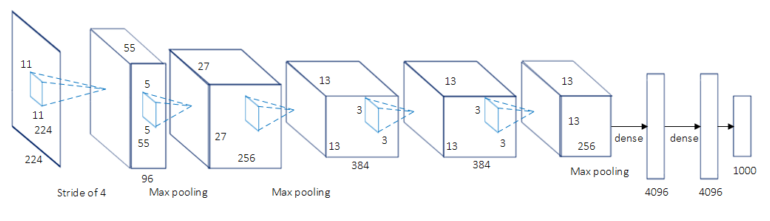
\includegraphics[width=0.7\linewidth]{fig/alexnet.png}
	\captionsource{AlexNet architecture}{\citeauthor{Krizhevsky2012}\cite{Krizhevsky2012}}
	\label{fig:alexnet}
\end{figure}


\subsection{VGG}
The Visual Geometry Group (VGG) model was introduced by the Visual Geometry Group at oxford university. In their paper, they propose multiple different architectural configurations with weight layers ranging from 13 - 16 layers deep. The most interesting is the model with 16 weight layers. It was submitted to ILSVRC 2013 and managed to get a top-5 test accuracy of 92.7\%. In \autoref{fig:vgg} we can see that the architecture makes us of more layers with small receptive fields rather than a few layers with large receptive fields.

\begin{figure}[H]
	\centering
	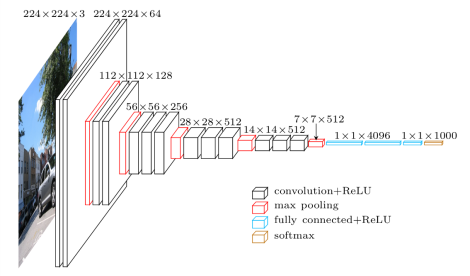
\includegraphics[width=0.7\linewidth]{fig/vgg16.png}
	\captionsource{VGG 16 architecture}{https://blog.heuritech.com/2016/02/29/a-brief-report-of-the-heuritech-deep-learning-meetup-5/}
	\label{fig:vgg}
\end{figure}


\subsection{GoogLeNet}
This network won the 2014 ILSVRC challenge with a top-5 test accuracy of 93.3\%. The network introduced a new architectural concept called the \emph{inception} model (see \autoref{fig:inceptionmodule}). The model is essentially a new mini-network with a pooling operation, large convolution layers, and smaller convolution layers. They proposed the use of small 1x1 convolution layers to reduce the complexity before the large convolution layers to keep the parameters and computational cost under control. This showed an increase in speed ranging from 3-10x faster than similar networks without the inception module.

\begin{figure}[H]
	\centering
	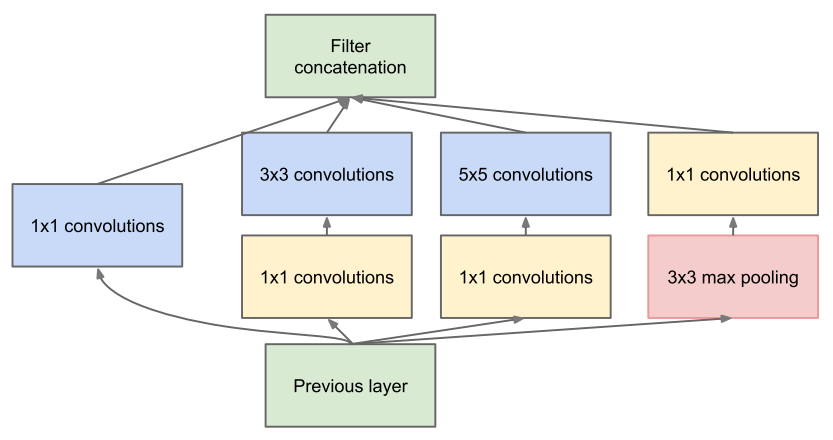
\includegraphics[width=0.7\linewidth]{fig/googlenet.png}
	\captionsource{Inception module}{\citeauthor{Szegedy2014}\cite{Szegedy2014}}
	\label{fig:inceptionmodule}
\end{figure}


\subsection{ResNet}
ResNet won the 2015 ILSVRC, with a top-5 test accuracy of 96.4\%. The network is known for its depth of 152 layers and a new kind of building block called residual block. The residual block contains two paths between the input and the output where one of the paths serve as a shortcut connection to the output (see \autoref{fig:residualblock}) essentially copying the input to the output layer. A big problem with very deep networks is that they are hard to optimize. When the depth of the network increases, the accuracy gets saturated. This is called \emph{degradation} and is the problem that the residual blocks are addressing by forcing the network to learn on top of already available input. 

\begin{figure}[H]
	\centering
	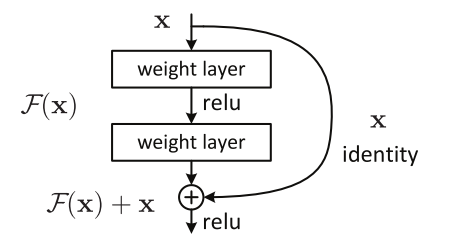
\includegraphics[width=0.5\linewidth]{fig/residual.png}
	\captionsource{Residual block.}{\citeauthor{He2015}\cite{He2015}}
	\label{fig:residualblock}
\end{figure}


\subsection{CapsNet}
Released November 2017, this is a very recent advancement in neural networks. It introduces a new type of neural network based on \emph{capsules}. 

BLABLABLA MORE ABOUT THIS

It addresses the issue that CNNs are not good at generalizing new viewpoints. They are good at generalizing to translation, but other affine transformations have shown to be difficult to learn. 


It has not (yet) been tested in ILSVRC but has been run on the Modified Institute of Standards and Technology database (MNIST) that is a database of handwritten digits. The database has 60000 training images and 10000 test images. 

\begin{figure}[H]
	\centering
	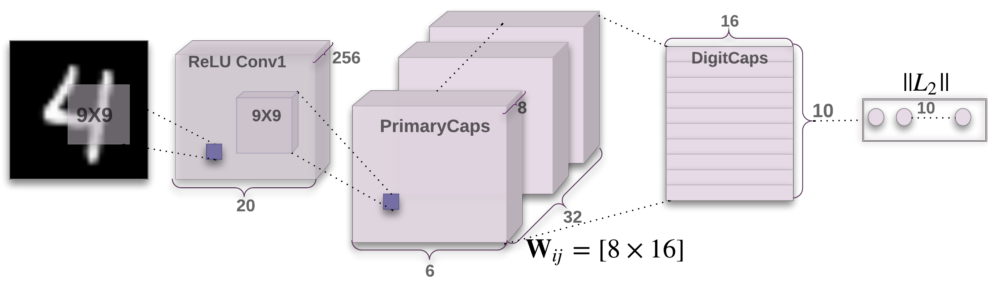
\includegraphics[width=0.7\linewidth]{fig/capsnet.png}
	\captionsource{CapsNet with 3 layers.}{\citeauthor{Sabour2017}\cite{Sabour2017}}
	\label{fig:capsnet}
\end{figure}


\section{Image segmentation}
Many of the previous network architectures described in \autoref{sec:important-architectures} are predicting labels of what the images contain and not where and what part of the image the labels are to be found in. Image segmentation is about assigning a class to each pixel with its enclosing object so we need output from the networks that are spatial maps instead of classification scores. In this section, we will review important networks that are specialized in image segmentation.


\subsection{FCN}
Fully Convolutional Network (FCN) by \citeauthor{Long2014} \cite{Long2014} can be seen as a common forerunner for semantic segmentation with convolutional networks \cite{Garcia-Garcia2017}. FCN adopted the contemporary deep classification nets AlexNet, VGG and GoogLeNet architectures we saw in \autoref{sec:important-architectures} to make dense predictions at the pixel level. It is important to note that they not only reused the architecture but used the pre-trained classification models as a starting point. The network replaced the fully-connected layers with convolutional ones, noting that the fully-connected layers could be seen as convolutional ones with kernels (filters) that cover the entire input region. This allowed segmentation maps to be generated from images of any size. Because of all the pooling operations in CNNs, a technique called \emph{deconvolution} \cite{Zeiler2011} was used to upsample the coarse output to dense pixels. Deconvolutional layers can learn interpolation functions the same way the network learns weights. Skip connections similar to the ones we saw in ResNet, are also included to give the deeper layers higher resolution feature maps.


\subsection{SegNet}





Dilated CONV
Deeplab v1 and v2
Refinenet
PSPnet
Large kernel Matters
Deeplab v3

 Texton forest 
 Random fort
 Patch
 FCN 2014
 U-NET
 CRF postprocessing
 

 
 EncoderDecoder